
\documentclass[10pt,letterpaper]{article}
\usepackage[top=0.85in,left=2.75in,footskip=0.75in]{geometry}

% amsmath and amssymb packages, useful for mathematical formulas and symbols
\usepackage{amsmath,amssymb}

% Use adjustwidth environment to exceed column width (see example table in text)
\usepackage{changepage}

% textcomp package and marvosym package for additional characters
\usepackage{textcomp,marvosym}

% cite package, to clean up citations in the main text. Do not remove.
\usepackage{cite}

% Use nameref to cite supporting information files (see Supporting Information section for more info)
\usepackage{nameref,hyperref}

% line numbers
\usepackage[right]{lineno}

% ligatures disabled
\usepackage[nopatch=eqnum]{microtype}
\DisableLigatures[f]{encoding = *, family = * }

% color can be used to apply background shading to table cells only
%\usepackage[table]{xcolor}

% array package and thick rules for tables
\usepackage{array}

% create "+" rule type for thick vertical lines
\newcolumntype{+}{!{\vrule width 2pt}}

% create \thickcline for thick horizontal lines of variable length
\newlength\savedwidth
\newcommand\thickcline[1]{%
  \noalign{\global\savedwidth\arrayrulewidth\global\arrayrulewidth 2pt}%
  \cline{#1}%
  \noalign{\vskip\arrayrulewidth}%
  \noalign{\global\arrayrulewidth\savedwidth}%
}

% \thickhline command for thick horizontal lines that span the table
\newcommand\thickhline{\noalign{\global\savedwidth\arrayrulewidth\global\arrayrulewidth 2pt}%
\hline
\noalign{\global\arrayrulewidth\savedwidth}}


% Remove comment for double spacing
%\usepackage{setspace} 
%\doublespacing

% Text layout
\raggedright
\setlength{\parindent}{0.5cm}
\textwidth 5.25in 
\textheight 8.75in

% Bold the 'Fig #' in the caption and separate it from the title/caption with a period
% Captions will be left justified
\usepackage[aboveskip=1pt,labelfont=bf,labelsep=period,justification=raggedright,singlelinecheck=off]{caption}
\renewcommand{\figurename}{Fig}

% Use the PLoS provided BiBTeX style
\bibliographystyle{plos2015}

% Remove brackets from numbering in List of References
\makeatletter
\renewcommand{\@biblabel}[1]{\quad#1.}
\makeatother



% Header and Footer with logo
\usepackage{lastpage,fancyhdr,graphicx}
\usepackage{epstopdf}
\usepackage{lmodern}
%\pagestyle{myheadings}
\pagestyle{fancy}
\fancyhf{}
%\setlength{\headheight}{27.023pt}
%\lhead{\includegraphics[width=2.0in]{PLOS-submission.eps}}
\rfoot{\thepage/\pageref{LastPage}}
\renewcommand{\headrulewidth}{0pt}
\renewcommand{\footrule}{\hrule height 2pt \vspace{2mm}}
\fancyheadoffset[L]{2.25in}
\fancyfootoffset[L]{2.25in}
\lfoot{\today}

%% Include all macros below

\newcommand{\lorem}{{\bf LOREM}}
\newcommand{\ipsum}{{\bf IPSUM}}

%% END MACROS SECTION

%% personal packages and macro
%%% packages
\usepackage[utf8]{inputenc}        % allow utf-8 input
\usepackage[T1]{fontenc}           % use 8-bit T1 fonts
\usepackage[dvipsnames, table]{xcolor}
\usepackage{tabularx}
\usepackage{multirow}
\usepackage{pifont}
\usepackage{csvsimple}
\usepackage[font={small},textfont={it},labelfont={bf}]{caption}
\usepackage{subcaption}
\usepackage{graphicx}
\usepackage{url}                   % simple URL typesetting
\usepackage{booktabs}              % professional-quality tables
\usepackage{makecell}
\usepackage{amsfonts}              % blackboard math symbols
\usepackage{amsmath}
\usepackage{nicefrac}              % compact symbols for 1/2, etc.
\usepackage{microtype}             % microtypography
\usepackage{enumitem}
\usepackage[export]{adjustbox}


%not compatible with cite package
%\usepackage[natbib=true,style=nature,maxnames=999,maxcitenames=2,backend=biber]{biblatex}
%\addbibresource{references.bib}

%%% macros
\DeclareMathOperator*{\argmin}{arg\,min}
\newcommand{\indep}{\perp \!\!\! \perp}
\newtheorem{assumption}{Assumption}

\definecolor{dark_blue}{rgb}{0,0,.65}
\definecolor{dark_green}{rgb}{0,.5,.15}

\hypersetup{pdftex,  % needed for pdflatex
  breaklinks=true,  % so long urls are correctly broken across lines
  colorlinks=true,
  linkcolor=dark_blue,
  citecolor=dark_green,
}
\colorlet{P}{ForestGreen}
\colorlet{I}{MidnightBlue}
\colorlet{C}{YellowOrange}
\colorlet{O}{DarkOrchid}
\colorlet{T}{Gray}



\begin{document}
\vspace*{0.2in}

\section*{Supporting information}


\paragraph*{S9 Fig}
\label{apd:vibration_analysis_for_aggregation}
{\bf Vibration analysis for aggregation.}

We conducted a dedicated vibration analysis on the different choices of
features aggregation, studying the impact on the estimated ATE. We also
studied if some choices of aggregation led to substantially poorer overlap.

We assessed overlap with two different methods. As recommended by
\cite{austin2015moving}, we did a graphical assessment by plotting the
distribution of the estimated. The treatment model hyper-parameters were chosen
by random search, then predicted propensity scores were obtained by refitting
this estimator with cross-fitting on the full dataset.

As shown in Fig \ref{apd:fig:albumin_for_sepsis:overlap_measure}, we did not find substantial differences between methods
when plotting graphically the distribution of the estimated propensity score.

\begin{figure}[h!]
    \centering
    \begin{subfigure}[b]{0.45\linewidth}
        \centering
        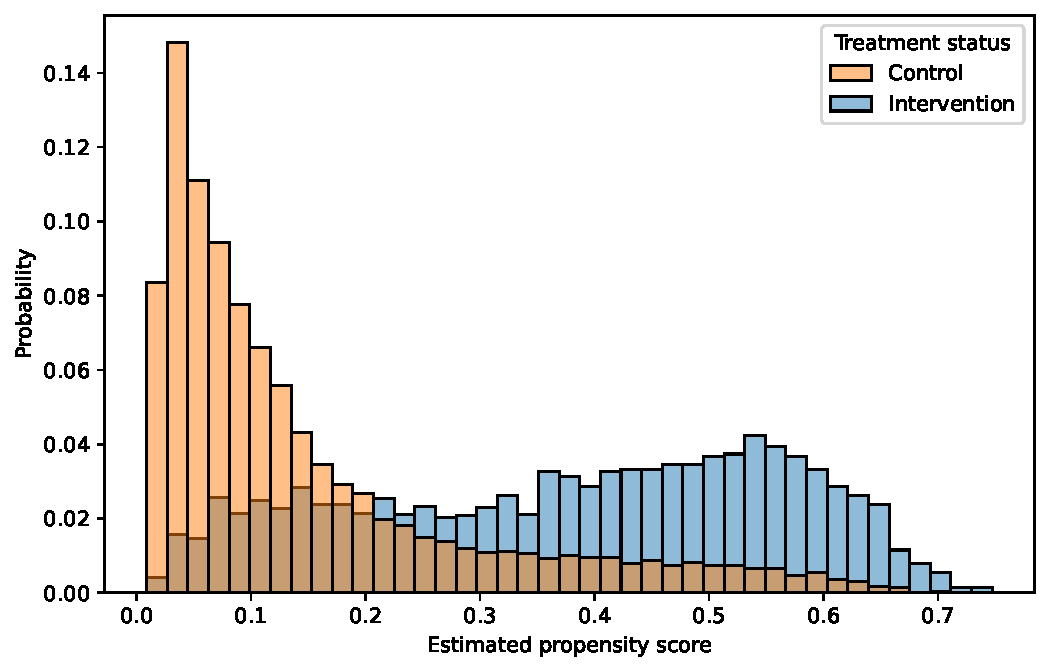
\includegraphics[width=\linewidth]{img_supp_final/sensitivity__ps_distribution__first_last_median__Forests.pdf}
        \caption{}\label{apd:fig:albumin_for_sepsis:overlap_measure_first_last_median}
    \end{subfigure}
    \hfill
    \begin{subfigure}[b]{0.45\linewidth}
        \centering
        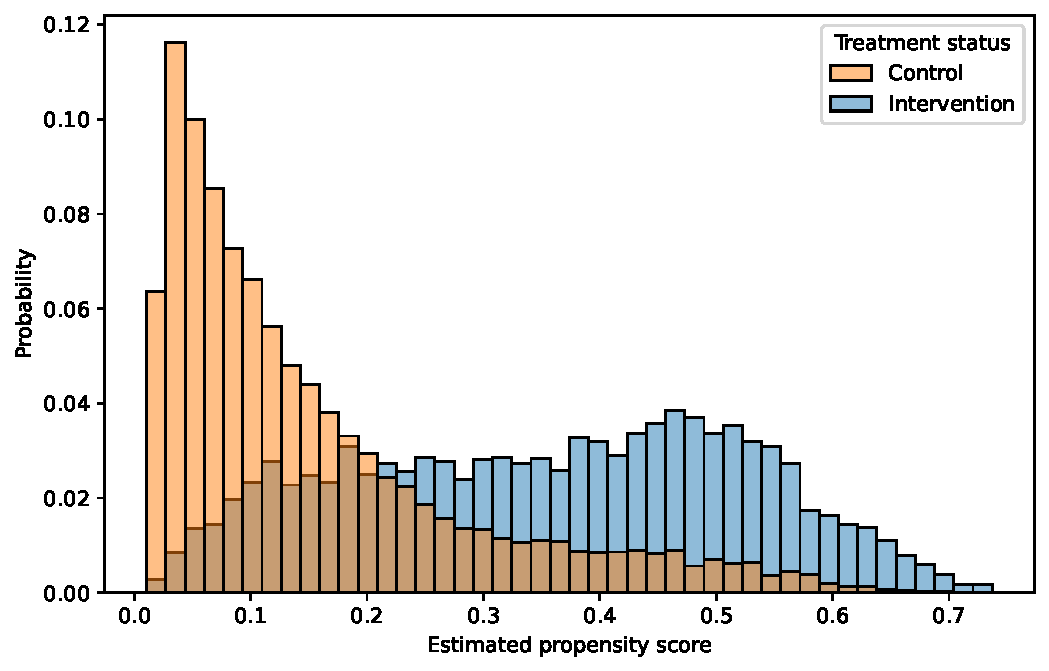
\includegraphics[width=\linewidth]{img_supp_final/sensitivity__ps_distribution__first__Forests.pdf}
        \caption{}\label{apd:fig:albumin_for_sepsis:overlap_measure_first}
    \end{subfigure}
    \caption{{\bf Different choices of aggregation yield qualitatively close
                distributions of the propensity score.}\\Fig
        \ref{apd:fig:albumin_for_sepsis:overlap_measure_first_last_median})a)
        shows a concatenation of first, last and median measures whereas Fig
        \ref{apd:fig:albumin_for_sepsis:overlap_measure_first})b) shows an
        aggregation by taking the first measure only. The underlying treatment
        effect estimator is a random forest. }\label{apd:fig:albumin_for_sepsis:overlap_measure}
\end{figure}

We also used normalized total variation (NTV) as a summary statistic of the
estimated propensity score to measure the distance between treated and control
population \cite{doutreligne2023select}. This statistic varies between 0 --
perfect overlap -- and 1 -- no overlap at all. Fig
\ref{apd:fig:albumin_for_sepsis:vibration_analysis_for_aggregation} shows no
marked differences in overlap as measured by NTV between aggregation choices,
comforting us in our expert-driven choice of the aggregation: a concatenation
of first and last feature observed before inclusion time.

\begin{figure}[h!]
    \centering
    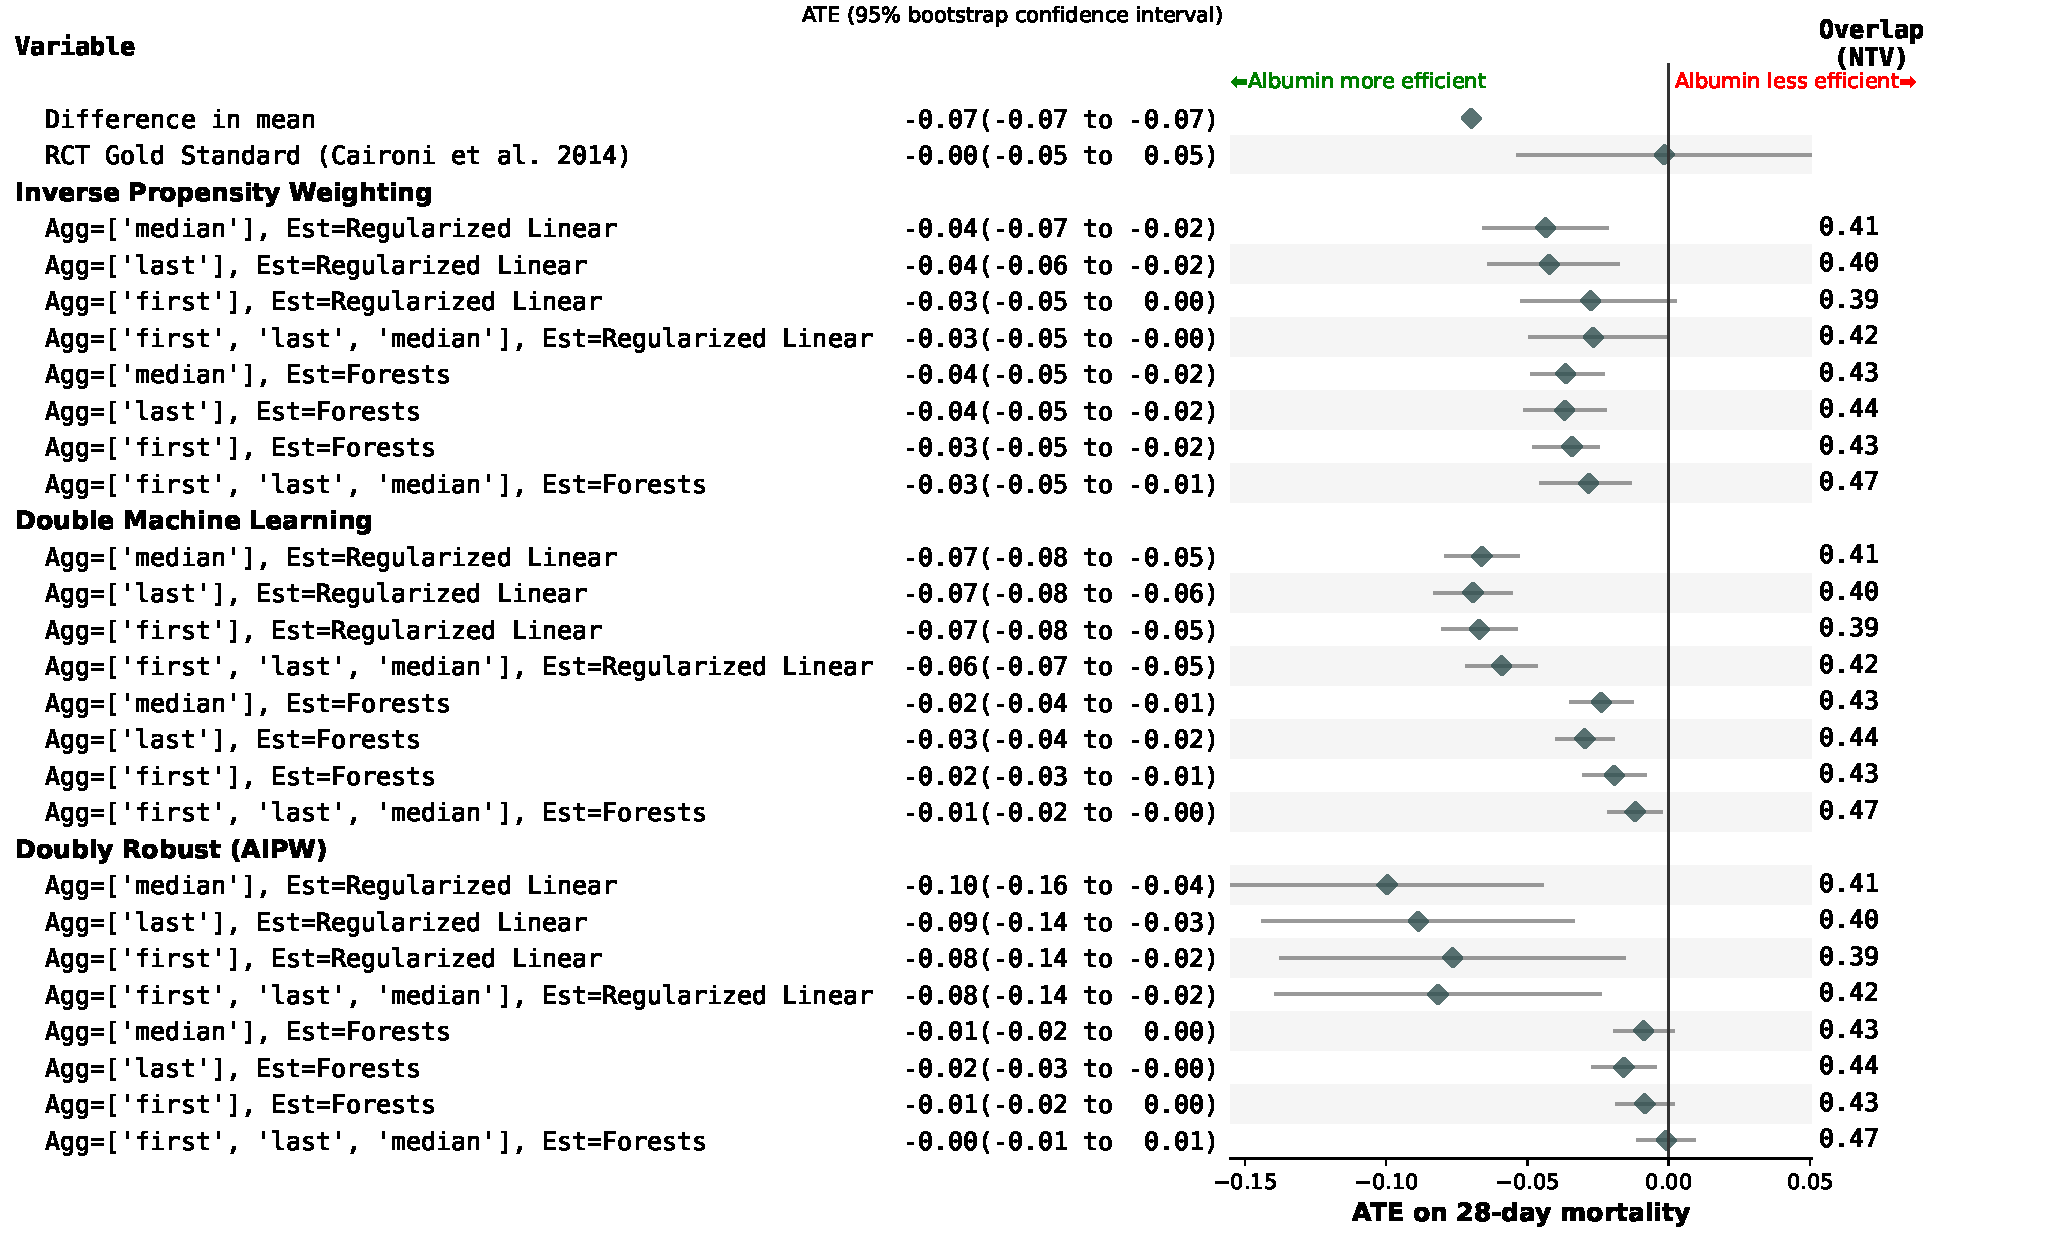
\includegraphics[width=1.0\linewidth]{img_supp_final/sensitivity_feature_aggregation_albumin_for_sepsis__bs_50.pdf}
    \caption{{\bf Vibration analysis dedicated to the aggregation choices.}\\The
        choices of aggregation only marginally modify the results. When assessed
        with Normalized Total Variation, the overlap assumption is respected for all
        our choices of aggregation. The green diamonds depict the mean effect and
        the bar are the 95\% confidence intervals obtained by 50 bootstrap
        repetitions.}\label{apd:fig:albumin_for_sepsis:vibration_analysis_for_aggregation}
\end{figure}


\bibliography{references}


\end{document}
